\section{Vorstellung Prototyp}
Nachfolgend folgt die Vorstellung des GUI-Prototypen des Business Transformation Trackers. Da dieser als Webanwendung konzeptiert ist, wurde auch der GUI-Protoyp an eine Webanwendung angelehnt. Der Prototyp erfüllt den Zweck die analysierten Anforderungen in einer grafischen Benutzeroberfläche abzubilden, um dem Auftraggeber und den Anwendern erste, leicht verständliche Einblicke in die Entwicklung zu geben. Dieser Prototyp dient einer späteren Umsetzung und Implementierung des BBT als Vorlage für die Benutzeroberfläche.

\subsubsection{Verwendete Werkzeuge}
Für die Entwicklung des Prototypen wurde auf das Programm Adobe XD zurückgegriffen. Dies entstammt dem Softwarehersteller Adobe und ist Teil der Softwaresuite \glqq{}Creative Cloud\grqq{}. Das Programm ist nur in einem Abonnement erhältich und kostet etwa 12 Euro im Monat. Mit Adobe XD ist eine Grafiksoftware mit der sich komplexe, grafische Benutzeroberflächen für unterschiedliche Bildschirmgrößen gestalten und zu einem animierten Prototypen überführen lassen.\footcite[Vgl.][]{adobe}


\subsubsection{Aufbau der Benutzeroberfläche}
Der Aufbau des Prototypen beginnt mit der Login-Fläche, die in Abbildung \ref{fig:Login} dargestellt ist. Auf dieser muss sich der Benutzer, im Falle einer späteren Implementierung, mit seinen persönlichen Benutzernamen und Kennwort anmelden.
\begin{figure}[h!]
    \centering
    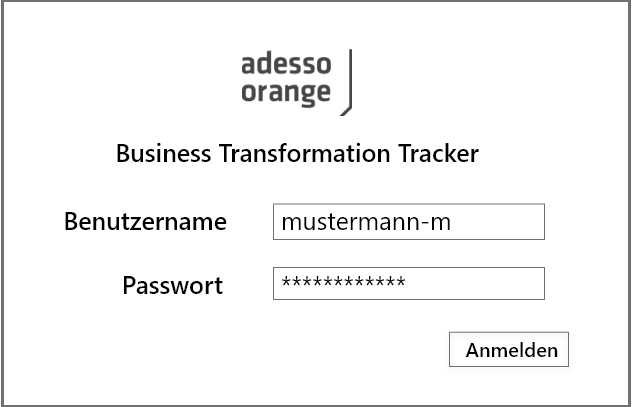
\includegraphics[scale=0.4]{./Prototyp/01_Login.png}
    \caption[Prototyp: Login-Bildschirm]{Login-Bildschirm}
    \label{fig:Login}
\end{figure}
\\Nachdem diese Anmeldung erfolgreich war, findet sich der Anwender auf der Startseite wieder, auf der er aktuelle Informationen über den Business Transformation Tracker und adesso orange vorfindet.
Auch sieht er hier zum ersten Mal den Aufbau, der sich durch die gesamte Benutzeroberfläche hinwegzieht. Bei der Gestaltung der Oberfläche wurde Wert auf ein \glqq{}Kachel-Design\grqq{} mit großen Schaltflächen gelegt, sodass die Oberfläche auf mobilen Endgeräten einfach zu verwenden ist. Bei der Farbgebung wurde sich für die Design-Farben von adesso orange beschrieben. Die Bedeutung der unterschiedlichen Farben in den Kacheln wird später erläutert. 
\begin{figure}[h!]
    \centering
    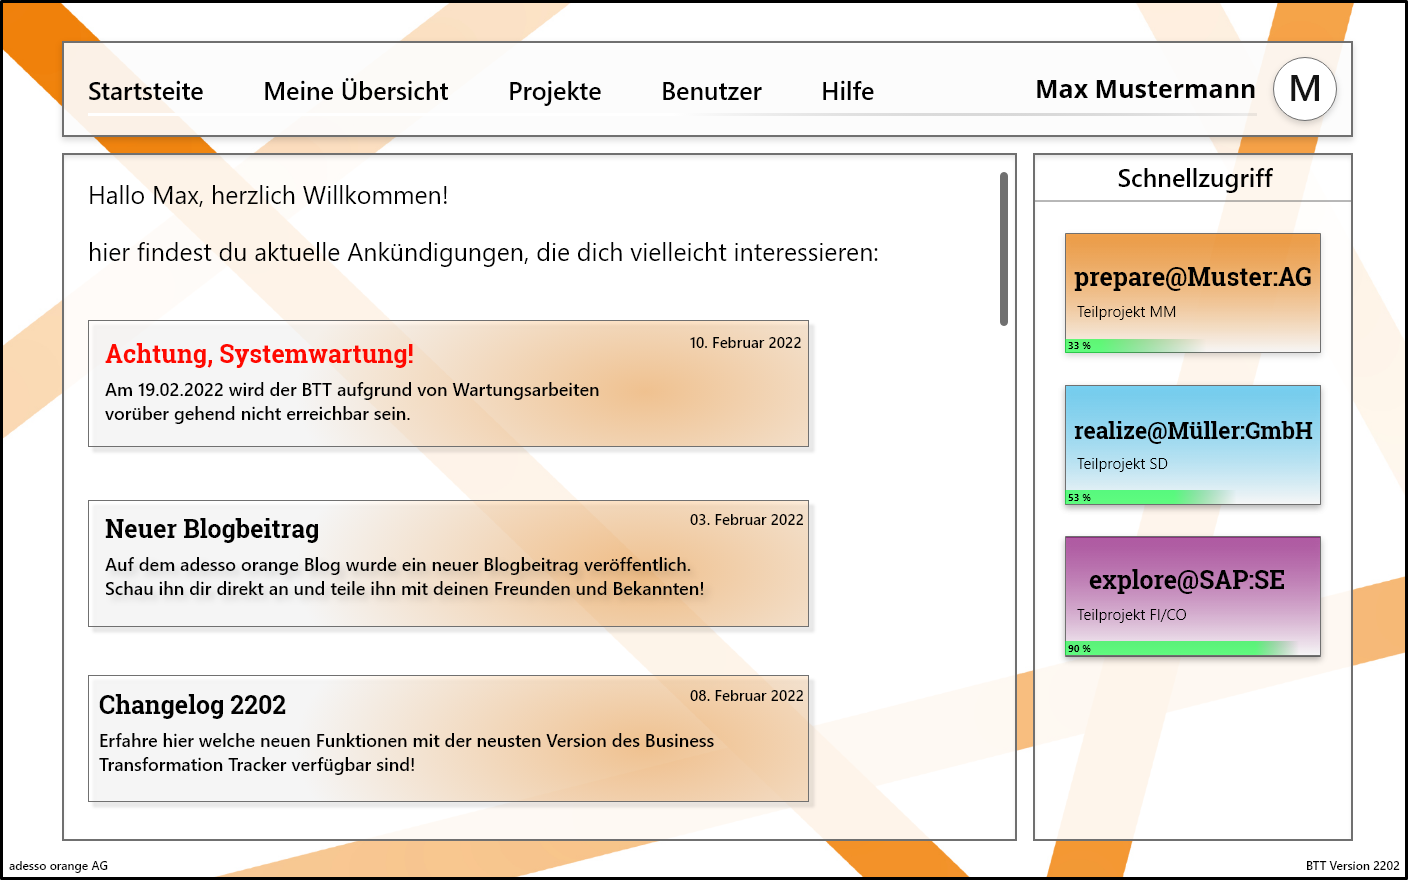
\includegraphics[scale=0.3]{./Prototyp/02_Startseite.png}
    \caption[Prototyp: Startseite]{Startseite}
    \label{fig:Startseite}
\end{figure}
\\Wie im Beispiel von Abbildung \ref{fig:Startseite} zu sehen, befindet sich im Kopf der Oberfläche ein Menü wieder, von dem aus der Benutzer stell auf die wichtigen Funktionen zugreifen kann. Mit dem Punkt \glqq{}Startseite\grqq{} gelangt er auf die hier dargestellte Startseite, mit dem Punkt \glqq{}Meine Übersicht\grqq{} gelangt der Benutzer auf eine Übersicht, in der er die ihm zugeordneten Projekte sehen kann, über den Menüpunkt \glqq{}Projekte\grqq{} und \glqq{}Benutzer\grqq{} jeweils auf die Projekt- und die Benutzerübersicht. Die Besonderheit an diesen Punkten ist, dass sie nur für die Rollen der Projektleiter und Administratoren sichtbar sind, damit nicht jeder Zugriff auf die personenbezogenen Daten und alle anderen Projekte erhält.\\Auf der rechten Seite befindet sich, abgetrennt vom Hauptfenster, ein kleineres Fenster mit der Übersicht Schnellzugriff. In diesem werden dem Benutzer seine eigenen, zugordneten, Projekte angezeigt, sowie das zugeordnete Teilprojekt und der Fortschrittsgrad des Teilprojekts.

\emph{Zur verbesserten Anschauung sind die Darstellungen des Prototypen ebenfalls im Verzeichnis ./Prototyp/ dieser Arbeit abgelegt. Dort sind ebenfalls drei Anwenungsfälle veranschaulicht.}\\